\section{Games as a Recursive Data Type}

We're going to characterize a special category \wnls\ of ``win-lose
games'' as a recursive data type and then prove, by structural
induction, a fundamental theorem about winning strategies for these
games.  The idea behind the recursive definition is to recognize that
the situation at any point during game play can itself be treated as
the start of a new game.  This is clearest for the game of Nim.

A Nim game starts with several piles of stones.  A move in the game
consists of removing some positive number of stones from a single
pile.  Two players alternate making moves, and whoever takes the last
stone wins.  For example, if there is only one pile, then the first
player to move wins by taking the whole pile.  On the hand, if the
game starts with just two piles, each with the same number of stones,
then the second player can guarantee a win simply by mimicking the
first player.  This means that if the first player removes three
stones from one pile, then the second player removes three stones from
the other pile.  At this point, it's worth thinking for a moment about
\textbf{why the mimicking strategy guarantees a win} for the second
player.







\subsection{Game Strategies}

A key question about a game is what strategy will give a player the best
score.  A \emph{strategy} for a player in a game specifies which move the
player should make at any point in the game.


\subsection{Game Trees}
More generally, we can describe the possible ways a game of Nim can be
played with a \term{game tree}.  A game tree for the Nim game that
starts with three piles of 3, 4 and 5 stones, respectively, is shown
in Figure~\ref{fig:endgame}.  The game tree has a \term{root} node
labelled with the starting position $\ang{3,4,5}$.\footnote{Game trees
  are usually pictured in this way, with the root at the top and lines
  connecting down to children.  The ``leaves'' at which the paths
  going down from the root appear at the bottom---in Computer as in
  geneaology, trees grow upside down.}  The root node is connected to
\emph{child nodes} corresponding to the possible piles after one move.
For example, the first player can remove between one and three stones
from the first pile leading to three possible piles of stones
\[
\ang{2,4,5},\ang{1,4,5},\ang{4,5}.
\]
Similarly, the first player has five possible ways to remove stones
from the last pile, leading to five possible piles of stones
\[
\ang{3,4,4}, \ang{3,4,3}, \ang{3,4,2}, \ang{3,4,1}, \ang{3,4} nodes.
\]
Altogether, the root of this particular game will be connected to $3
\times 4 \times 5 = 60$ child nodes.

Each child node will now have grandchild nodes showing the possible
piles of stones after the second player moves.  For example, the child
node $\ang{3,4,1}$ will be connected to $3 \times 4 \times 1 = 12$
grandchild nodes.  A path following connections down from the root to
a leaf describes a complete \term{play} of the game.\footnote{In
  English, ``Nim game'' might refer to the rules that define the game,
  but it might also refer to a particular play---as in the once famous
  third game in the 1961 movie \emph{Last Year at Marienbad}.  It's
  usually easy to figure out which way the phrase is being used, and
  we won't worry about it.}

\begin{figure}[htbp]
%\graphic{endgame}
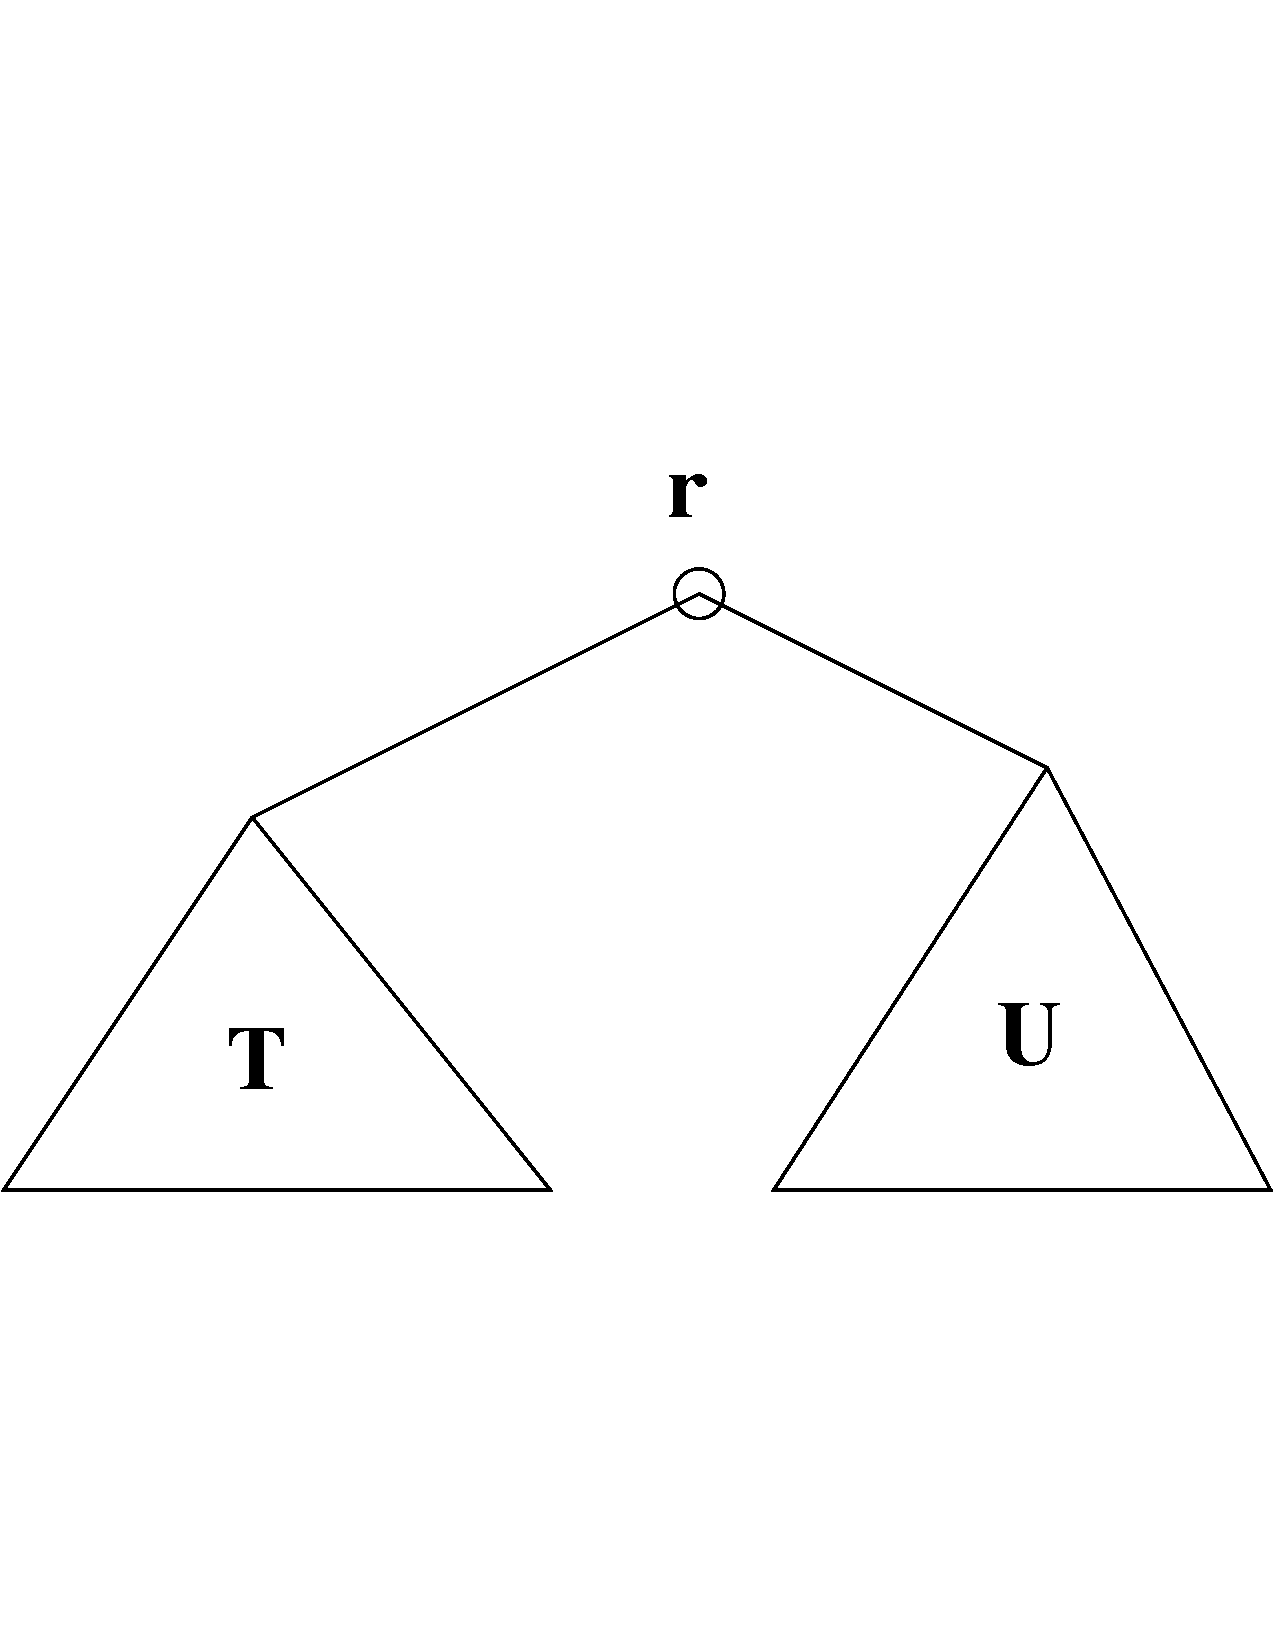
\includegraphics[width=6in]{recBST.pdf} %nimtree
\caption{\TBA{Game Tree for Nim starting with three piles of sizes $\ang{5,5,7}$}.}
\label{fig:endgame}
\end{figure}




\subsection{Who has the Winning Strategy?}
Notice that although Theorem~\ref{fund} guarantees a winning strategy, its
proof gives no clue which player has it.  For the Subset Takeaway Game of
Problem~\ref{CP_subset_take_away} and most familiar $\tg$'s like Chess,
Go, \dots, no one knows which player has a winning
strategy.\footnote{Checkers used to be in this list, but there has been a
  recent announcement that each player has a strategy that forces a tie.
  (reference TBA)}

%% Games as a Recursive Data Type Problems %%%%%%%%%%%%%%%%%%%%%%%%%%%%%%%%%%%%
\begin{problems}
\practiceproblems
\pinput{TP_Game_trees}

\homeworkproblems
\pinput{PS_VG}
\pinput{PS_nim_strategy}
\end{problems}

\begin{editingnotes}
\section{Rules for Quantifiers}

\subsection{Prenex Form}
\begin{problems}
\pinput{CP_variable_convention}
\pinput{CP_prenex}
\pinput{CP_recursive_prenex}
\pinput{PS_recursive_variable_convention}
\end{problems}
\end{editingnotes}

%% Induction in Computer Science %%%%%%%%%%%%%%%%%%%%%%%%%%%%%%%%%%%%%%%%%%%%%%
\section{Induction in Computer Science}
\index{induction}

Induction is a powerful and widely applicable proof technique, which
is why we've devoted two entire chapters to it.  Strong induction and
its special case of ordinary induction are applicable to any kind of
thing with nonnegative integer sizes---which is an awful lot of things,
including all step-by-step computational processes.

Structural induction then goes beyond number counting, and offers a
simple, natural approach to proving things about recursive data types
and recursive computation.

In many cases, a nonnegative integer size can be defined for a recursively
defined datum, such as the length of a string, or the number of operations
in an $\aexp$.  It is then possible to prove properties of data by ordinary
induction on their size.  But this approach often produces more cumbersome
proofs than structural induction.

In fact, structural induction is theoretically more powerful than ordinary
induction.  However, it's only more powerful when it comes to reasoning
about infinite data types---like infinite trees, for example---so this
greater power doesn't matter in practice.  What does matter is that for
recursively defined data types, structural induction is a simple and
natural approach.    This makes it a technique every computer
scientist should embrace.

\endinput

%%%%%%%%%%%%%%%%%%%%%%%%%%%%%%%%%%%%%%%%%%%%%%%


\begin{editingnotes}

\section{Tagged data}

Labelling a recursively defined data item with a tag that uniquely
determines the rule used to construct it is a standard approach to
avoiding ambiguous recursive definitions in programming.  This
amounts to working with data items that are already \term{parsed}, that
is, represented as \term{parse trees}.

For example, the parse tree for the arithmetic expression
\begin{equation}\label{ax}
-(a(x\cdot x)+ bx) + 1
\end{equation}
is shown in Figure~\ref{fig:parse}.

\begin{figure}
%\graphic{parsetree}
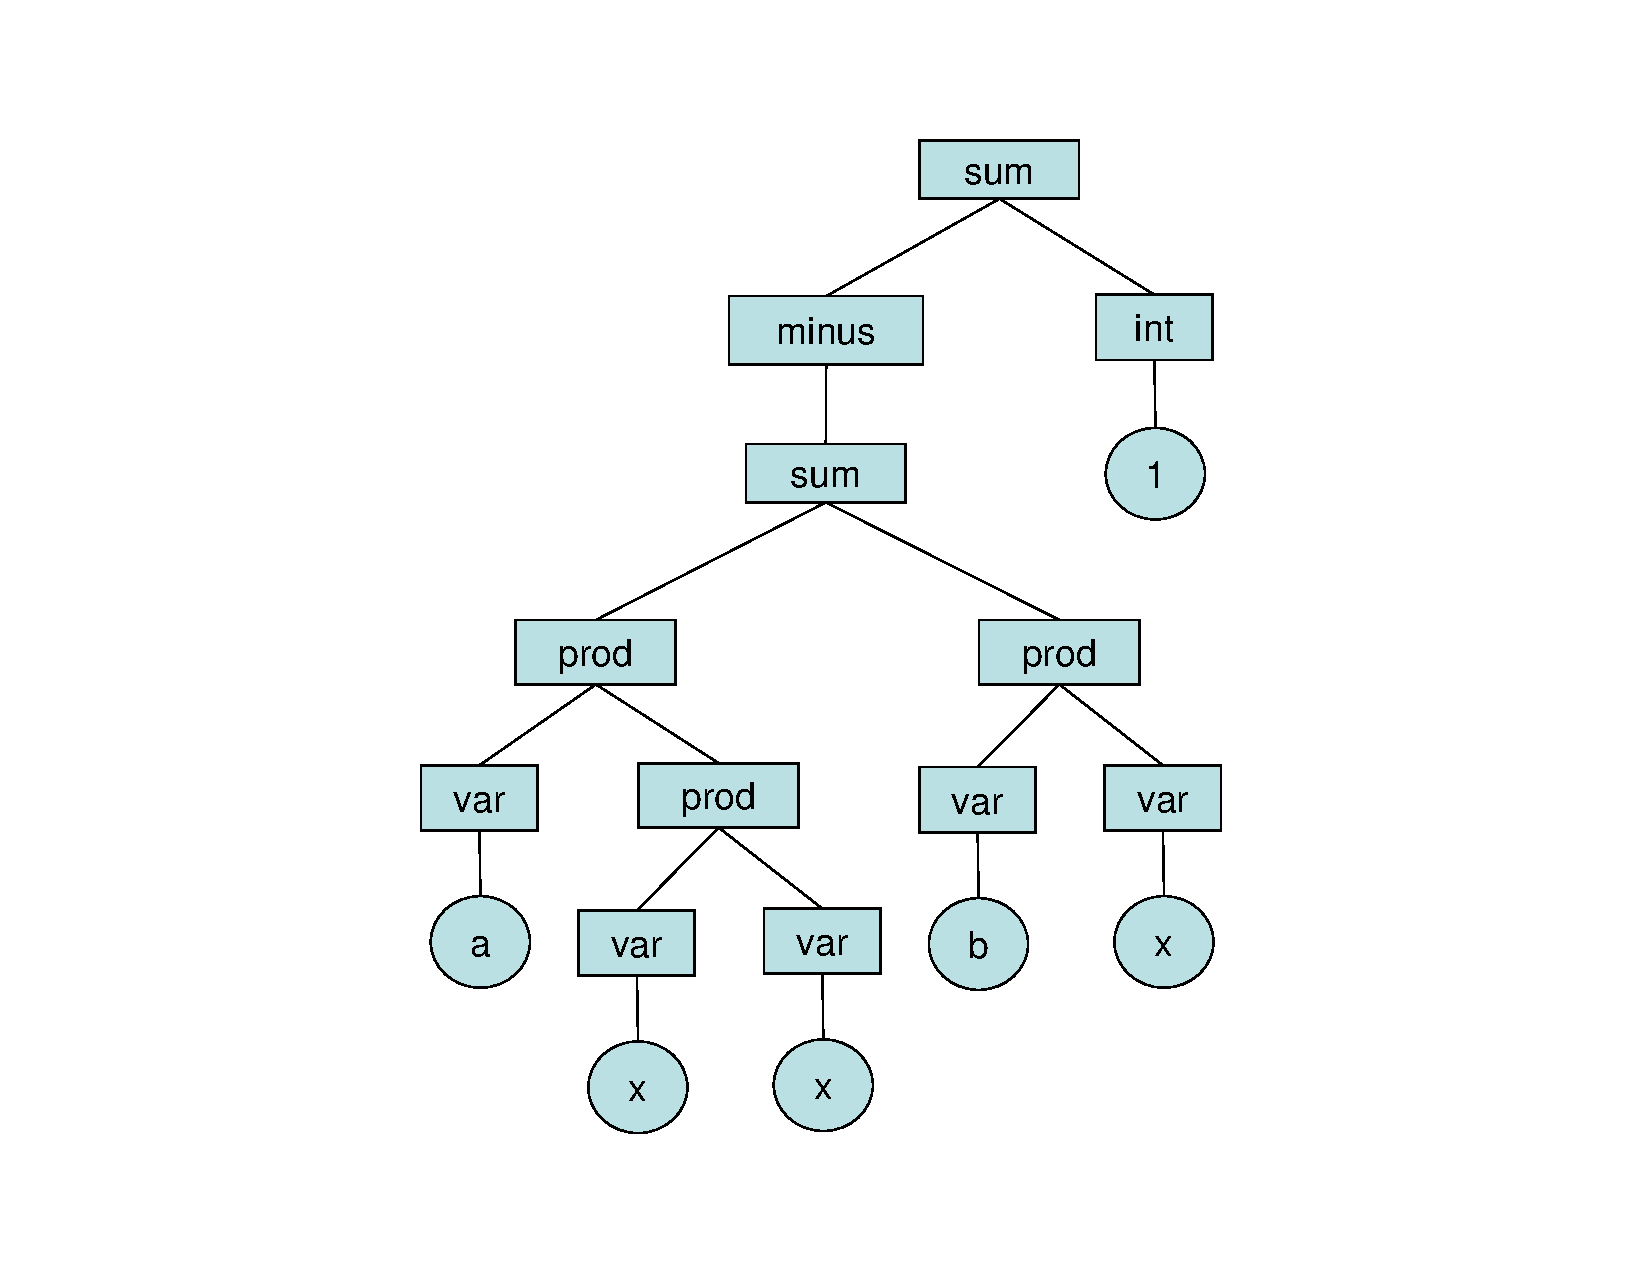
\includegraphics[width=5in]{parsetree}
\caption{Parse tree for $-(a(x\cdot x)+ bx) + 1$.}
\label{fig:parse}
\end{figure}

In a computer, such a tree would be represented by pairs or triples
that begin with a
\emph{tag} equal to the label of the top node of the parse tree.  
The general definition of parse trees for $\aexp$'s would be:

%\newcommand{\paexp}{\text{Aexp-parse-tree}}

\begin{definition}\label{arithparse}
The set $\paexp$ of \emph{parse trees for arithmetic expressions} 
over a set of
\emph{variables} $V$ is defined recursively as follows:
\begin{itemize}
\item \inductioncase{Base cases}:
\begin{enumerate}
\item If $n \in \integers$, then $\ang{\texttt{int}, n} \in \paexp$.
\item If $v \in V$, then $\ang{\texttt{var}, v} \in \paexp$.
\end{enumerate}
\item \inductioncase{Constructor cases}: if $e,e' \in \paexp$, then
\begin{enumerate}
\item $\ang{\texttt{sum}, e, e'} \in \paexp$,
\item $\ang{\texttt{prod}, e, e'} \in \paexp$, and
\item $\ang{\texttt{minus}, e} \in \paexp$.
\end{enumerate}
\end{itemize}
\end{definition}

So the $\paexp$ corresponding to formula~\ref{ax} would be:
\begin{equation}\label{axtag}
\begin{array}{rll}
\left< \right. \texttt{sum}, 
         & \left< \right. \texttt{minus},\ \ \left< \right. \texttt{sum},
               & \ang{\texttt{prod},\ \ \ang{\texttt{var},\ a},
                                     \ang{\texttt{prod},\ \
                                            \ang{\texttt{var},\ x},\
                                            \ang{\texttt{var},\ x}}},\\
                               && \left. \left. \ang{\texttt{prod},\ \
                                       \ang{\texttt{var},\ b},\
                                       \ang{\texttt{var},\ x}}
                                   \right> \right>,\\
         & \left. \left. \ang{\texttt{int},\ 1} \right> \right>
\end{array}
\end{equation}
Now the expression~\ref{ax} is certainly a lot more humanly
intelligible than~\ref{axtag}, but~\ref{axtag} is in the
representation best suited and commonly used in compiling and
processing computer programs.

\end{editingnotes}

\endinput


\begin{editingnotes}

\subsection{A String Theorem}

Here is a more complex proof, illustrating a combination of structural
induction and strengthening the hypothesis.

\begin{theorem}
  In a string of $0$s and $1$s, the number of occurrences of the pattern
  $01$ is less than or equal to the number of occurrences of $10$, plus
  one.
\end{theorem}

Let's try to prove this by structural induction.  First we must
define $P(s)$.  Let's write $\ms{num}(pat,s)$ as the number of
occurrences of the pattern string pat in s.  Now our inductive
hypothesis is
\[
P(s): \ms{num}(01,s) \leq \ms{num}(10,s) + 1. 
\]
If you try to prove this by structural induction, you will get
stuck.
Why? 
Consider what happens when you add $1$ at the end.  
This could increase the number of $01$s without increasing the number of
$10$s. 

So, to prove by structural induction on strings, let's strengthen the
hypothesis by adding another clause.  If a string ends in $0$ then
the number of $01$s is less than or equal to the number of $10$s.
That solves the problem by weakening what we have to show when the
string ends in $1$.  But maybe it causes another problem somewhere
else.  Let's give it a try:

Redefine $P(s) \eqdef$
\begin{eqnarray*}
\ms{num}(01,s) & \leq & \ms{num}(10,s) + 1, \text{ and}\\
\lefteqn{\text{If $s$ ends in $0$ then}}\\
\ms{num}(01,s) & \leq  &\ms{num}(10,s).
\end{eqnarray*} 
 
This means that, for each inductive step have two things to show.

First let's consider $s1$. This is the case that looks dangerous,
because it might increase the number of $01$s.  We have to prove two
statements.  The second is easy, because the new string doesn't end in
$0$.  We say it's ``vacuously true''.

The first statement now takes some work. 
We might be adding to the number of $01$s.  
However, if we do, the previous string must have ended with $0$. 
Then the inductive hypothesis says that the previous string had to
satisfy the stronger inequality in the second statement. 
Adding one to the LHS of the stronger inequality yields the weaker
inequality we want.

The following proof fragment considers cases based on whether $s$ ends
in $0$ or not.  If not, it might end in $1$, or might be empty (don't
forget this possibility).

Of course, you could also expand the step for $s$ ending in $1$ into a
careful series of inequalities.

Now consider $s0$.  We hope that what we did to make the $s1$ case
work doesn't mess up the $s0$ case.  But we have to check.

The first statement is easy.  It follows from the first statement of
the inductive hypothesis for $s$, because we are not increasing the
number of $01$s.  But now the second statement takes more work.  The
difficulty is that the new string ends in $0$, which means that we
have to show the stronger inequality in the second statement.  But to
do this, we might only have the weaker inequality for the previous
string.  The argument again depends on what the previous string $s$
ended with.  So again, we consider cases, based on whether $s$ ends in
$0$ or $1$, or is empty.  If $s$ ends in $0$ we rely on the second
statement of the inductive hypothesis for $s$ (with the stronger
inequality), whereas if $s$ ends in $1$ we rely on the first statement
(with the weaker inequality).  In this case, we have to ``turn the
weaker inequality into the stronger inequality''.

If you actually write out all these cases in the proof, you will
notice that some facts are stated repeatedly, e.g., that when you add
a $0$ to the end of a string you are not increasing the number of
$01$s.  To avoid having to state these facts several times, you can
move them earlier in the proof.

\end{editingnotes}

\iffalse

\subsection{Tic-Tac-Toe}
Tic-Tac-Toe is a game for young children.  There are two players who
alternately write the letters ``X'' and ``O'' in the empty boxes of a
$3 \times 3$ grid.  A grid pattern with three of the same letter
filling a row, column, or diagonal is called a \emph{tic-tac-toe}, and
the first player who gets a tic-tac-toe of their letter wins the game.
Children generally don't take long to figure out an optimal strategy
for playing the game.

We can diagram the ways to play Tic-Tac-Toe using a Tic-Tac-Toe game
tree.  The game tree starts with a \emph{root node} labelled with the
empty $3 \times 3$ grid.  This node then connects directly to
``child'' nodes labelled with each of the different grid patterns
possible after the first move.  According to Tic-Tac-Toe rules, the
X-player gets to move first, so the root of the tree connects directly
to nine different child nodes, each labelled with a different one of
the nine grid patterns containing one X and eight empty boxes.  Each
of these one-X child nodes connects in turn to eight child nodes of
its own labelled with the eight different one-X/one-O grid
patterns possible after the second player puts an O in a box.  These
move possibilities are given by the Tic-Tac-Toe \emph{game tree}
illustrated in Figure~\ref{fig:Tic-Tac-Toe}.
\fi

\begin{editingnotes}
This could be simplified by having who moves first be defined by the
game itself.  Then a game has only one value, namely, the max value
that the max player can ensure---which equals the minimum value that
the min-player can hold down.
\end{editingnotes}

\iffalse
In particular, there are two players called the \term{max-player} and the
\term{min-player} who alternate making moves.  The score measures what the
max-player wins (it might be negative, indicating that the min-player came
out ahead).  The objective of the max-player is to have play end with as
high a score as possible, while the min-player aims to end with as low a
score as possible.

Given which of the players moves first in a game, a strategy for the
max-player is said to \emph{ensure} the payoff $s$ if play ends with a
score $ \ge k$, no matter what moves the min-player makes.  Likewise, a
strategy for the min-player is said to \emph{hold down} the score to $s$,
if play ends with a payoff of $\le s$, no matter what moves the max-player
makes.

A $\tg$ has two values: a \term{max value} and a \term{min value}.
The \emph{max value} is $s$ if the max-player has a strategy that
ensures payoff $s$, and the min-player has a strategy that holds down
the payoff to $s$, when the \emph{max-player moves first}.  Likewise,
the $\tg$ has \emph{min value} $s$, if the same thing holds when the
\emph{min-player moves first}.

The \emph{Fundamental Theorem} for 2-person 50-point games of perfect
information is that is that every game has both a max value and a min
value.  (Note: the two values are usually different.)

What this means is that there's no point in playing a game: if the max
player gets the first move, the min-player should just pay the max-player
the max value of the game without bothering to play (a negative payment
means the max-player is paying the min-player).  Likewise, if the
min-player gets the first move, the min-player should just pay the
max-player the min value of the game.

PPART\label{finpg} Prove this Fundamental Theorem for 50-valued
$\tg$'s by structural induction.

SOLUTION

The proof is by structural induction on the definition of a
  $\tg$ $G$.  The induction hypothesis is that there is that
\begin{quote}
  $G$ has a max value and a min value.
\end{quote}

\inductioncase{Base case}: [$G$ is the terminated game with payoff $k$].  The only
possible play is $k$.  So the max value and the min value are both $k$.

\inductioncase{Constructor case}: [$G = (G_0,\dots, G_n)$].  By structural
induction we may assume that each of the games $G_i$ have both max values
and min values.

We first show that $G$ has max value $k$ where $k$ is the largest min
value among the games $G_0,\dots,G_n$.

To prove the max value of $G$ is $k$, we must show how the max-player,
moving first in $G$, can ensure $k$, and how the min-player, moving second
in $G$, can hold down the payoff to $k$.

To ensure $k$, the max-player simply chooses $i$ as her first move where
game $G_i$ has this largest min value $k$.  The min-player then has the
first move in $G_i$, so by definition of min value, the max-player has a
strategy in $G_i$ that ensures $k$, which she can now follow.  So this
first move, combined with the ensuring strategy in $G_i$, defines a
strategy for the max-player in $G$ that ensures $k$.

Likewise, there is a simple strategy for the min-player, moving second in
$G$, to hold down the payoff to $k$.  Namely, suppose the max-player's
first move is $i$.  Then $G_i$ has a min value of $m \leq k$, since $k$ is
the largest min value.  So by definition of min value, there is a strategy
in $G_i$ for the min-player to hold down the payoff to $m$, which he can
now follow, thereby holding down the payoff of play on $G$ to $m \leq k$.

The existence of these ensuring and holding down strategies for $G$
implies that the max value of $G$ is $k$.

Second, to show that $G$ has a min value, we can repeat the previous
argument with min and max exchanged.

Therefore, by structural induction, we can conclude that all $\tg$'s have
min and max values.

SOLUTION

PPART A meta-$\tg$ game has as possible first moves the choice of
\emph{any} $\tg$ to play.  Meta-$\tg$ games aren't any harder to
understand than $\tg$'s, but there is one notable difference, they
have an infinite number of possible first moves.  We could also define
meta-meta-$\tg$'s in which the first move was a choice of any
$\tg$ \emph{or} the meta-$\tg$ game to play.  In
meta-meta-$\tg$'s there are an infinite number of possible first
\emph{and} second moves.  And then there's $\text{meta}^3-\tg$ \dots.

\iffalse
The 2D-origin game in a Week 4 class problem is a game in which there are
an infinite number of possible first moves, an infinite number of possible
second moves, \dots.  \iffalse (with two values, ``win'' or ``lose''
instead of values from -50 to 50)\fi
\fi

To model such infinite games, we could have modified the recursive
definition of $\tg$'s to allow first moves that choose any one of an
infinite sequence
\[
G_0,G_1,\dots,G_n,G_{n+1}, \dots
\]
of $\tg$'s.  Now a $\tg$ can be a mind-bendingly infinite datum
instead of a finite one.

Do these infinite $\tg$'s still have max and min values?  In
particular, do you think it would be correct to use structural induction
as in part~\eqref{finpg} to prove a Fundamental Theorem for such infinite
$\tg$'s?  Offer an answer to this question, and briefly indicate why
you believe in it.

SOLUTION

It may not be obvious, but structural induction is a perfectly sound proof
technique even for infinite recursively defined data, and the proof of the
Fundamental Theorem for $\tg$'s applies without change to infinite ones.

SOLUTION

\begin{theorem}\label{fund}
  \textbf{Fundamental Theorem for Two-Person Games:} For every two-person
  terminating game of perfect information, has a max-value and a
  min-value.
\end{theorem}

\begin{proof}
The proof is by structural induction on the definition of a $\tg$ $G$.
The induction hypothesis is that there is a winning strategy for $G$.

\inductioncase{Base cases}:
\begin{enumerate}

\item $G=\ang{\textbf{leaf}, \textbf{win}}$.  Then the first player has the
 winning strategy: ``make the winning move.''

\item $G=\ang{\textbf{leaf}, \textbf{lose}}$.  Then the second player has a
 winning strategy: ``Let the first player make the losing move.''
\end{enumerate}

\inductioncase{Constructor case}: Suppose $G = \ang{\textbf{tree},\mathcal{G}}$.
By structural induction, we may assume that some player has a winning
strategy for each $G' \in \mathcal{G}$.  There are two cases to consider:
\begin{itemize}
\item some $G_0 \in \mathcal{G}$ has a winning strategy for its second
  player.  Then the first player in $G$ has a winning strategy: make the
  move to $G_0$ and then follow the second player's winning strategy in
  $G_0$.

\item every $G' \in \mathcal{G}$ has a winning strategy for its first
  player.  Then the second player in $G$ has a winning strategy: if the
  first player's move in $G$ is to $G_0 \in \mathcal{G}$, then follow the
  winning strategy for the first player in $G_0$.
\end{itemize}
So in any case, one of the players has a winning strategy for $G$, which
completes the proof of the constructor case.

It follows by structural induction that there is a winning strategy for
every $\tg$ $G$.
\end{proof}
\fi

\iffalse
\begin{figure}
%\graphic{topgame}
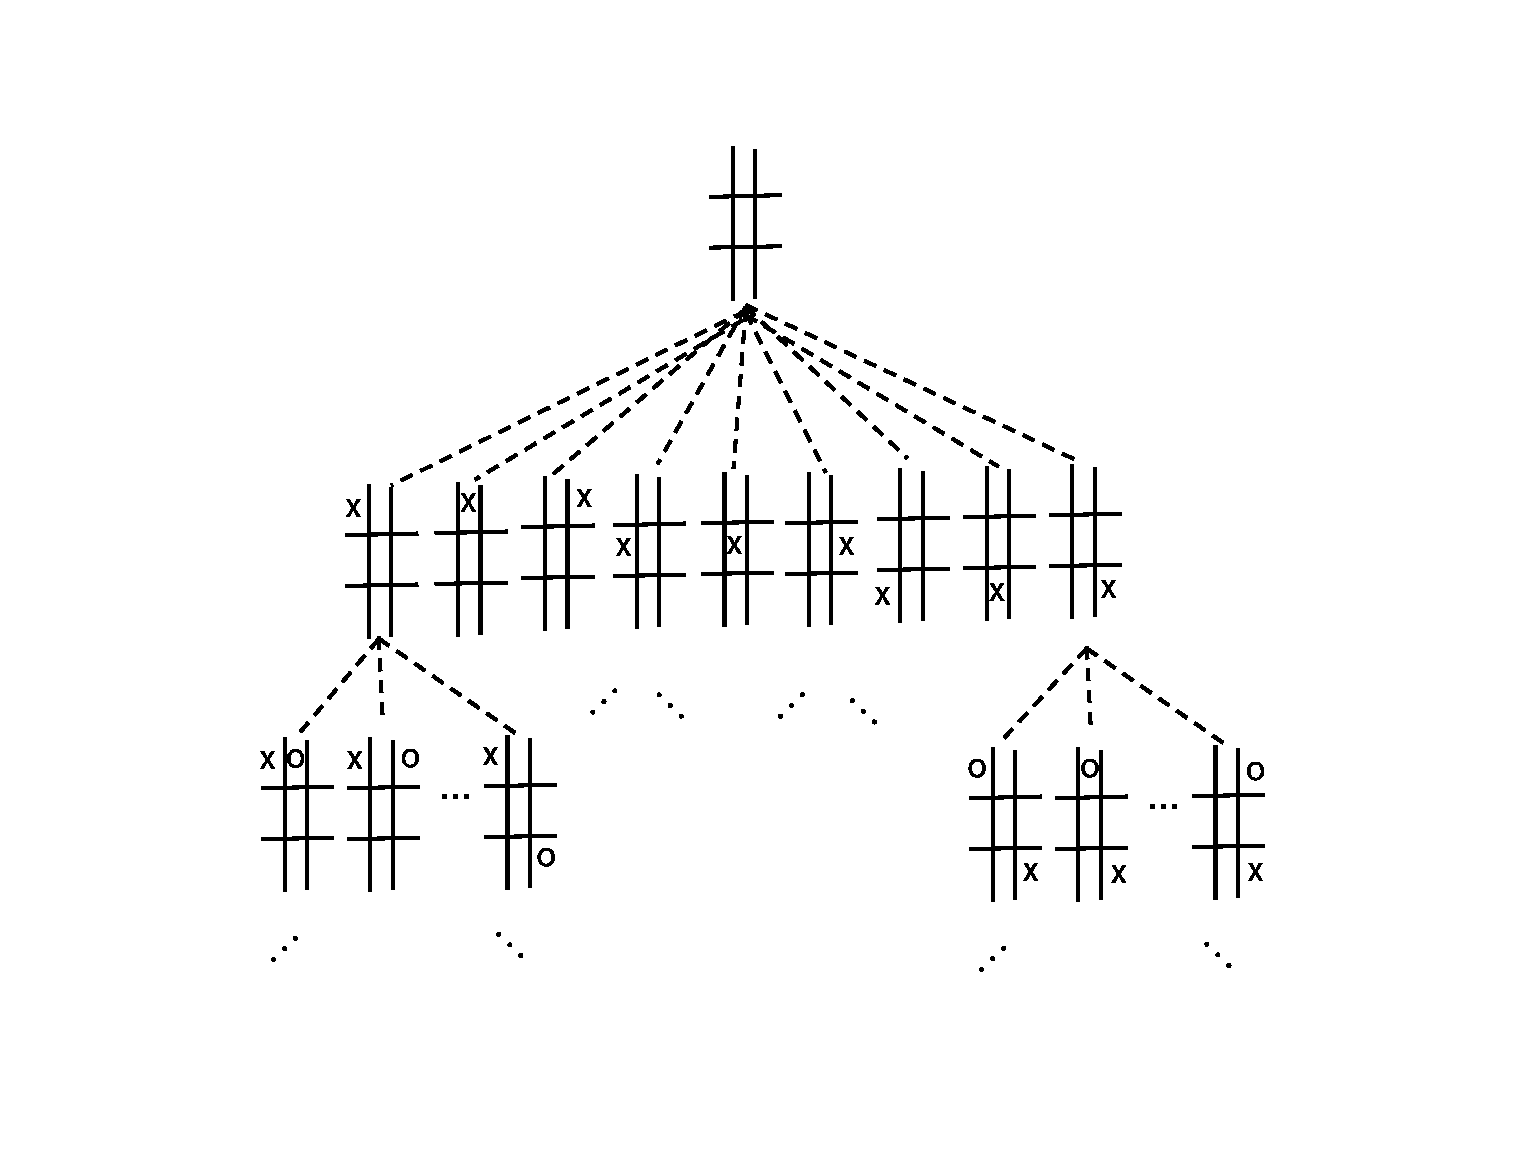
\includegraphics[width=6.5in]{topgame}
\caption{The Top of the Game Tree for Tic-Tac-Toe.}
\label{fig:Tic-Tac-Toe}
\end{figure}

The construction of the tree continues with each second move node
connecting to third level child nodes labelled with each of the seven
two-X, one-O patterns possible after the next move, and so on.  This
continues until all that's left are ``leaf'' nodes labelled with
\emph{terminated} patterns from which there is no further legal move.
The \term{terminated patterns} are those either containing a
three-in-a-row tic-tac-toe or else without any empty boxes.  (Quickie:

what is the highest level at which not every node has the the same
number of child nodes?)

The game tree embodies the rules and all the possible ways of playing
Tic-Tac-Toe.  It also illustrates another idea: each node in the tree
is the root of its tree of descendent of nodes.  This leads us to the
definition of the recursive data type of Tic-Tac-Toe trees.

\begin{definition}
The Tic-Tac-Toe game trees are defined recursively as follows:

\inductioncase{Base Case}: If $P$ is a terminated grid pattern, then a
single node labelled $P$ is a Tic-Tac-Toe tree.  This node is the root
of the tree and is also defined to be a \term{leaf} of the tree.

\inductioncase{Constructor case}: If $P$ is a non-terminated
Tic-Tac-Toe pattern, let $\mathcal{T}$ be a set of Tic-Tac-Toe game
trees whose roots are labelled with the distinct grid patterns
possible after one move from $P$.  Moreover, no node appears in
different trees in $\mathcal{T}$.  Then a tree with a root node not in
$\mathcal{T}$ and labelled $P$ whose child nodes are the roots of the
trees in $\mathcal{T}$, is a Tic-Tac-Toe game tree.  Its leaves are
the leaves of all the trees in $\mathcal{T}$.

\end{definition}

For example, for grid patterns
\begin{align*}
P_0 & =  \tbegin{array}{c|c|c}
                O & X & O\\
         \hline X & O & X\\
         \hline X & &
        \end{array}\\
Q_1 & = \begin{array}{c|c|c}
                O & X & O\\
         \hline X & O & X\\
         \hline X &  & O
        \end{array}\\
Q_2 & = \begin{array}{c|c|c}
                O & X & O\\
         \hline X & O & X\\
         \hline X & O & 
        \end{array}\\
R & = \begin{array}{c|c|c}
                O & X & O\\
         \hline X & O & X\\
         \hline X & O & X
        \end{array}
\end{align*}
a game tree with root labelled $P_0$ is pictured in Figure~\ref{fig:endgame}.
\fi



\begin{editingnotes}

\subsection{A String Theorem}

Here is a more complex proof, illustrating a combination of structural
induction and strengthening the hypothesis.

\begin{theorem}
  In a string of $0$s and $1$s, the number of occurrences of the pattern
  $01$ is less than or equal to the number of occurrences of $10$, plus
  one.
\end{theorem}

Let's try to prove this by structural induction.  First we must
define $P(s)$.  Let's write $\ms{num}(pat,s)$ as the number of
occurrences of the pattern string pat in s.  Now our inductive
hypothesis is
\[
P(s): \ms{num}(01,s) \leq \ms{num}(10,s) + 1. 
\]
If you try to prove this by structural induction, you will get
stuck.
Why? 
Consider what happens when you add $1$ at the end.  
This could increase the number of $01$s without increasing the number of
$10$s. 

So, to prove by structural induction on strings, let's strengthen the
hypothesis by adding another clause.  If a string ends in $0$ then
the number of $01$s is less than or equal to the number of $10$s.
That solves the problem by weakening what we have to show when the
string ends in $1$.  But maybe it causes another problem somewhere
else.  Let's give it a try:

Redefine $P(s) \eqdef$
\begin{eqnarray*}
\ms{num}(01,s) & \leq & \ms{num}(10,s) + 1, \text{ and}\\
\lefteqn{\text{If $s$ ends in $0$ then}}\\
\ms{num}(01,s) & \leq  &\ms{num}(10,s).
\end{eqnarray*} 
 
This means that, for each inductive step have two things to show.

First let's consider $s1$. This is the case that looks dangerous,
because it might increase the number of $01$s.  We have to prove two
statements.  The second is easy, because the new string doesn't end in
$0$.  We say it's ``vacuously true''.

The first statement now takes some work. 
We might be adding to the number of $01$s.  
However, if we do, the previous string must have ended with $0$. 
Then the inductive hypothesis says that the previous string had to
satisfy the stronger inequality in the second statement. 
Adding one to the LHS of the stronger inequality yields the weaker
inequality we want.

The following proof fragment considers cases based on whether $s$ ends
in $0$ or not.  If not, it might end in $1$, or might be empty (don't
forget this possibility).

Of course, you could also expand the step for $s$ ending in $1$ into a
careful series of inequalities.

Now consider $s0$.  We hope that what we did to make the $s1$ case
work doesn't mess up the $s0$ case.  But we have to check.

The first statement is easy.  It follows from the first statement of
the inductive hypothesis for $s$, because we are not increasing the
number of $01$s.  But now the second statement takes more work.  The
difficulty is that the new string ends in $0$, which means that we
have to show the stronger inequality in the second statement.  But to
do this, we might only have the weaker inequality for the previous
string.  The argument again depends on what the previous string $s$
ended with.  So again, we consider cases, based on whether $s$ ends in
$0$ or $1$, or is empty.  If $s$ ends in $0$ we rely on the second
statement of the inductive hypothesis for $s$ (with the stronger
inequality), whereas if $s$ ends in $1$ we rely on the first statement
(with the weaker inequality).  In this case, we have to ``turn the
weaker inequality into the stronger inequality''.

If you actually write out all these cases in the proof, you will
notice that some facts are stated repeatedly, e.g., that when you add
a $0$ to the end of a string you are not increasing the number of
$01$s.  To avoid having to state these facts several times, you can
move them earlier in the proof.

\end{editingnotes}


\begin{editingnotes}
This could be simplified by having who moves first be defined by the
game itself.  Then a game has only one value, namely, the max value
that the max player can ensure---which equals the minimum value that
the min-player can hold down.
\end{editingnotes}

\iffalse
In particular, there are two players called the \term{max-player} and the
\term{min-player} who alternate making moves.  The score measures what the
max-player wins (it might be negative, indicating that the min-player came
out ahead).  The objective of the max-player is to have play end with as
high a score as possible, while the min-player aims to end with as low a
score as possible.

Given which of the players moves first in a game, a strategy for the
max-player is said to \emph{ensure} the payoff $s$ if play ends with a
score $ \ge k$, no matter what moves the min-player makes.  Likewise, a
strategy for the min-player is said to \emph{hold down} the score to $s$,
if play ends with a payoff of $\le s$, no matter what moves the max-player
makes.

A $\tg$ has two values: a \term{max value} and a \term{min value}.
The \emph{max value} is $s$ if the max-player has a strategy that
ensures payoff $s$, and the min-player has a strategy that holds down
the payoff to $s$, when the \emph{max-player moves first}.  Likewise,
the $\tg$ has \emph{min value} $s$, if the same thing holds when the
\emph{min-player moves first}.

The \emph{Fundamental Theorem} for 2-person 50-point games of perfect
information is that is that every game has both a max value and a min
value.  (Note: the two values are usually different.)

What this means is that there's no point in playing a game: if the max
player gets the first move, the min-player should just pay the max-player
the max value of the game without bothering to play (a negative payment
means the max-player is paying the min-player).  Likewise, if the
min-player gets the first move, the min-player should just pay the
max-player the min value of the game.

PPART\label{finpg} Prove this Fundamental Theorem for 50-valued
$\tg$'s by structural induction.

SOLUTION

The proof is by structural induction on the definition of a
  $\tg$ $G$.  The induction hypothesis is that there is that
\begin{quote}
  $G$ has a max value and a min value.
\end{quote}

\inductioncase{Base case}: [$G$ is the terminated game with payoff $k$].  The only
possible play is $k$.  So the max value and the min value are both $k$.

\inductioncase{Constructor case}: [$G = (G_0,\dots, G_n)$].  By structural
induction we may assume that each of the games $G_i$ have both max values
and min values.

We first show that $G$ has max value $k$ where $k$ is the largest min
value among the games $G_0,\dots,G_n$.

To prove the max value of $G$ is $k$, we must show how the max-player,
moving first in $G$, can ensure $k$, and how the min-player, moving second
in $G$, can hold down the payoff to $k$.

To ensure $k$, the max-player simply chooses $i$ as her first move where
game $G_i$ has this largest min value $k$.  The min-player then has the
first move in $G_i$, so by definition of min value, the max-player has a
strategy in $G_i$ that ensures $k$, which she can now follow.  So this
first move, combined with the ensuring strategy in $G_i$, defines a
strategy for the max-player in $G$ that ensures $k$.

Likewise, there is a simple strategy for the min-player, moving second in
$G$, to hold down the payoff to $k$.  Namely, suppose the max-player's
first move is $i$.  Then $G_i$ has a min value of $m \leq k$, since $k$ is
the largest min value.  So by definition of min value, there is a strategy
in $G_i$ for the min-player to hold down the payoff to $m$, which he can
now follow, thereby holding down the payoff of play on $G$ to $m \leq k$.

The existence of these ensuring and holding down strategies for $G$
implies that the max value of $G$ is $k$.

Second, to show that $G$ has a min value, we can repeat the previous
argument with min and max exchanged.

Therefore, by structural induction, we can conclude that all $\tg$'s have
min and max values.

SOLUTION

PPART A meta-$\tg$ game has as possible first moves the choice of
\emph{any} $\tg$ to play.  Meta-$\tg$ games aren't any harder to
understand than $\tg$'s, but there is one notable difference, they
have an infinite number of possible first moves.  We could also define
meta-meta-$\tg$'s in which the first move was a choice of any
$\tg$ \emph{or} the meta-$\tg$ game to play.  In
meta-meta-$\tg$'s there are an infinite number of possible first
\emph{and} second moves.  And then there's $\text{meta}^3-\tg$ \dots.

\iffalse
The 2D-origin game in a Week 4 class problem is a game in which there are
an infinite number of possible first moves, an infinite number of possible
second moves, \dots.  \iffalse (with two values, ``win'' or ``lose''
instead of values from -50 to 50)\fi
\fi

To model such infinite games, we could have modified the recursive
definition of $\tg$'s to allow first moves that choose any one of an
infinite sequence
\[
G_0,G_1,\dots,G_n,G_{n+1}, \dots
\]
of $\tg$'s.  Now a $\tg$ can be a mind-bendingly infinite datum
instead of a finite one.

Do these infinite $\tg$'s still have max and min values?  In
particular, do you think it would be correct to use structural induction
as in part~\eqref{finpg} to prove a Fundamental Theorem for such infinite
$\tg$'s?  Offer an answer to this question, and briefly indicate why
you believe in it.

SOLUTION

It may not be obvious, but structural induction is a perfectly sound proof
technique even for infinite recursively defined data, and the proof of the
Fundamental Theorem for $\tg$'s applies without change to infinite ones.

SOLUTION

\begin{theorem}\label{fund}
  \textbf{Fundamental Theorem for Two-Person Games:} For every two-person
  terminating game of perfect information, has a max-value and a
  min-value.
\end{theorem}

\begin{proof}
The proof is by structural induction on the definition of a $\tg$ $G$.
The induction hypothesis is that there is a winning strategy for $G$.

\inductioncase{Base cases}:
\begin{enumerate}

\item $G=\ang{\textbf{leaf}, \textbf{win}}$.  Then the first player has the
 winning strategy: ``make the winning move.''

\item $G=\ang{\textbf{leaf}, \textbf{lose}}$.  Then the second player has a
 winning strategy: ``Let the first player make the losing move.''
\end{enumerate}

\inductioncase{Constructor case}: Suppose $G = \ang{\textbf{tree},\mathcal{G}}$.
By structural induction, we may assume that some player has a winning
strategy for each $G' \in \mathcal{G}$.  There are two cases to consider:
\begin{itemize}
\item some $G_0 \in \mathcal{G}$ has a winning strategy for its second
  player.  Then the first player in $G$ has a winning strategy: make the
  move to $G_0$ and then follow the second player's winning strategy in
  $G_0$.

\item every $G' \in \mathcal{G}$ has a winning strategy for its first
  player.  Then the second player in $G$ has a winning strategy: if the
  first player's move in $G$ is to $G_0 \in \mathcal{G}$, then follow the
  winning strategy for the first player in $G_0$.
\end{itemize}
So in any case, one of the players has a winning strategy for $G$, which
completes the proof of the constructor case.

It follows by structural induction that there is a winning strategy for
every $\tg$ $G$.
\end{proof}
\fi

\iffalse
\begin{figure}
%\graphic{topgame}
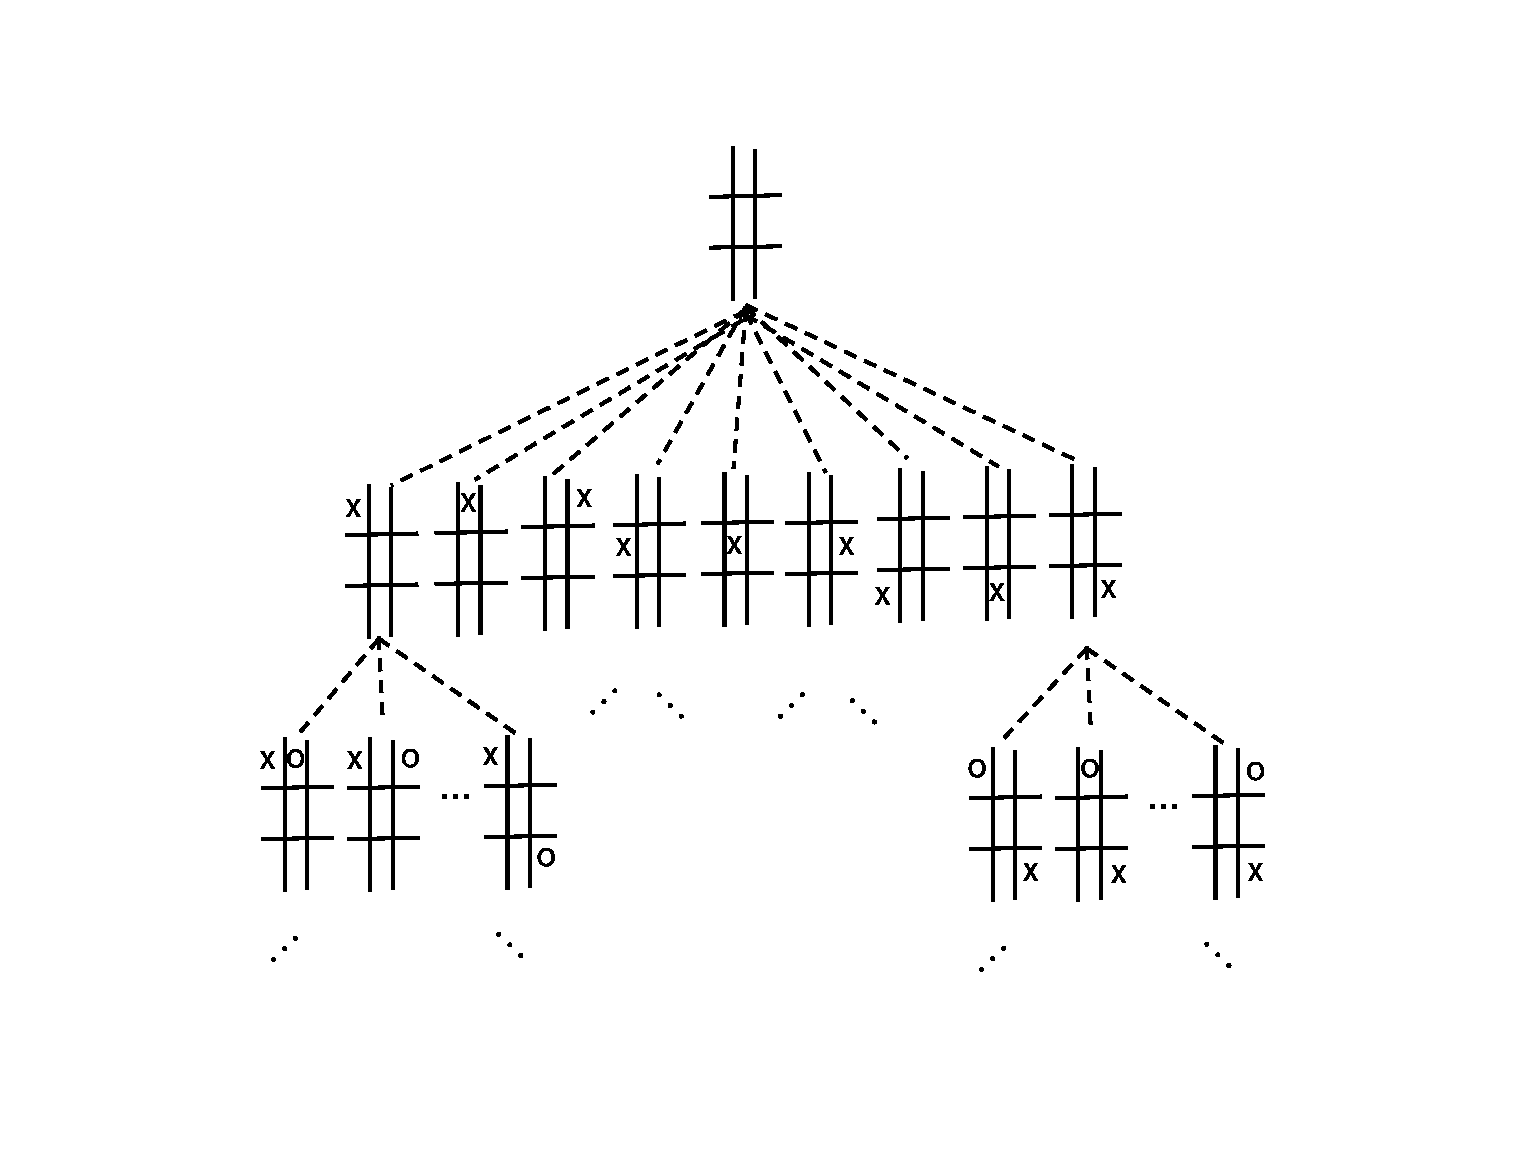
\includegraphics[width=6.5in]{topgame}
\caption{The Top of the Game Tree for Tic-Tac-Toe.}
\label{fig:Tic-Tac-Toe}
\end{figure}

The construction of the tree continues with each second move node
connecting to third level child nodes labelled with each of the seven
two-X, one-O patterns possible after the next move, and so on.  This
continues until all that's left are ``leaf'' nodes labelled with
\emph{terminated} patterns from which there is no further legal move.
The \term{terminated patterns} are those either containing a
three-in-a-row tic-tac-toe or else without any empty boxes.  (Quickie:

what is the highest level at which not every node has the the same
number of child nodes?)

The game tree embodies the rules and all the possible ways of playing
Tic-Tac-Toe.  It also illustrates another idea: each node in the tree
is the root of its tree of descendent of nodes.  This leads us to the
definition of the recursive data type of Tic-Tac-Toe trees.

\begin{definition}
The Tic-Tac-Toe game trees are defined recursively as follows:

\inductioncase{Base Case}: If $P$ is a terminated grid pattern, then a
single node labelled $P$ is a Tic-Tac-Toe tree.  This node is the root
of the tree and is also defined to be a \term{leaf} of the tree.

\inductioncase{Constructor case}: If $P$ is a non-terminated
Tic-Tac-Toe pattern, let $\mathcal{T}$ be a set of Tic-Tac-Toe game
trees whose roots are labelled with the distinct grid patterns
possible after one move from $P$.  Moreover, no node appears in
different trees in $\mathcal{T}$.  Then a tree with a root node not in
$\mathcal{T}$ and labelled $P$ whose child nodes are the roots of the
trees in $\mathcal{T}$, is a Tic-Tac-Toe game tree.  Its leaves are
the leaves of all the trees in $\mathcal{T}$.

\end{definition}

For example, for grid patterns
\begin{align*}
P_0 & =  \tbegin{array}{c|c|c}
                O & X & O\\
         \hline X & O & X\\
         \hline X & &
        \end{array}\\
Q_1 & = \begin{array}{c|c|c}
                O & X & O\\
         \hline X & O & X\\
         \hline X &  & O
        \end{array}\\
Q_2 & = \begin{array}{c|c|c}
                O & X & O\\
         \hline X & O & X\\
         \hline X & O & 
        \end{array}\\
R & = \begin{array}{c|c|c}
                O & X & O\\
         \hline X & O & X\\
         \hline X & O & X
        \end{array}
\end{align*}
a game tree with root labelled $P_0$ is pictured in Figure~\ref{fig:endgame}.
\fi



\begin{figure}[htbp]
\graphic{endgame}
\includegraphics[width=6in]{nimtree}
\caption{\TBA{Game Tree for Nim starting with three piles of sizes $\ang{5,5,7}$}.}
\label{fig:endgame}
\end{figure}

Game trees are usually pictured in this way, with the root at the top
and lines connecting down to children.  So the leaves appear at the
bottom of the tree---in Computer and geneaology, trees grow upside
down.  A path following connections down from the root to a leaf
describes a complete \term{play} of the game.

\begin{editingnotes}
In English, ``Tic-Tac-Toe game'' might refer to the rules that define
Tic-Tac-Toe, the representation of those rules in the Tic-Tac-Toe game
tree whose root is labelled with an empty grid.  But ``Tic-Tac-Toe
game'' might also refer to a particular play, as in describing
yesterday's exciting Tic-Tac-Toe game.  It's usually easy to figure
out which way the phrase is being used, so we won't worry about this.
\end{editingnotes}


\begin{editingnotes}
\subsection{Infinite Tic-Tac-Toe Games}
At any point in a Tic-Tac-Toe game, there are at most nine possible
next patterns, and no play can continue for more than nine moves.  But
we can expand Tic-Tac-Toe into a larger game by running a 5-game
tournament: play Tic-Tac-Toe five times and the tournament winner is
the player who wins the most individual games.  A 5-game tournament
can run for as many as 45 moves.

It's not much of generalization to have an \emph{$n$-game Tic-Tac-Toe
  tournament}.  But then comes a generalization that sounds simple but can
be mind-boggling: consolidate all these different size tournaments into a
single game we can call \emph{Tournament-Tic-Tac-Toe ($T^4$)}.  The first
player in a game of $T^4$ chooses any integer $n > 0$.  Then the players
play an $n$-game tournament.  Now we can no longer say how long a $T^4$
play can take.  In fact, there are $T^4$ plays that last as long as you
might like: if you want a game that has a play with, say, nine billion
moves, just have the first player choose $n$ equal to one billion.  This
should make it clear the game tree for $T^4$ is infinite.

But still, it's clear that every possible $T^4$ play will stop.
That's because after the first player chooses a value for $n$, the
game can't continue for more than $9n$ moves.  So it's not possible to
keep playing forever even though the game tree is infinite.

This isn't very hard to understand, but there is an important
difference between any given $n$-game tournament and $T^4$: even
though every play of $T^4$ must come to an end, there is no longer any
initial bound on how many moves it might be before the game ends---a
play might end after 9 moves, or $9(2001)$ moves, or $9(10^{10}+1)$
moves.  It just can't continue forever.

While there is no bound on how long to play, at least after the
first move to an $n \times n$ board in meta-Tic-Tac-Toe, we know the game
will end with $n^2$ moves.

Now that we recognize $T^4$ as a \tg, we can go on to
a \emph{meta}-$T^4$ game, where the first player chooses a number,
$m>0$, of $T^4$ games to play, and then the second player gets the
first move in each of the individual $T^4$ games to be played.

Then, of course, there's meta-meta-$T^4$\dots.

Every play of the meta-meta game must still end, but now even
after the first move, there is no bound on how long a game might
continue.
\end{editingnotes}

\subsection{Two Person Terminating Games}

Familiar games like Tic-Tac-Toe, Checkers, and Chess can be assigned
scores of 1, -1, or 0 corresponding to win, lose, or draw.  The game of Go
is often scored by counting the difference in the numbers of locations
controlled by the two players.  An $n$-game tournament of win, lose draw
games might be scored by adding up the scores of the individual games,
which would equal the number of games won by the first player minus the
number they lost.  \iffalse A negative score would mean the second player
won more games.\fi

The idea behind the definition of $\tg$'s as a recursive data type is that
making a move in a $\tg$ leads to the start of a subgame, as in Tic-Tac-Toe.  So
given any set of games, we can make a new game whose first move is to pick a
game to play from the set.  At the end of play there is a score.

So what defines a game?  For Tic-Tac-Toe, we used the patterns and the
rules of Tic-Tac-Toe to determine the next patterns.  But once we have
a complete game tree, we don't really need the pattern labels: the
root of a game tree itself can play the role of a ``board position''
with its possible ``next positions'' determined by the roots of its
subtrees.  So any game is defined by its game tree.  This leads to the
following very simple---perhaps deceptively simple---general
definition.

\begin{definition}\label{tgdef}
  Let $S$ be a set of real numbers whose members will be called
  \emph{scores}. The \emph{game trees for $S$-scored two-person
    terminating games of perfect information} are defined recursively as
  follows:
\begin{itemize}

\item \inductioncase{Base case}:
\[
\ang{\textbf{leaf}, s} \in \tg,
\]
for all $s \in S$.

\item \inductioncase{Constructor case}:
If $\mathcal{G}$ is a nonempty set of
$\tg$'s, then $G$ is a $\tg$, where
\[
G \eqdef \ang{\textbf{tree},\mathcal{G}}.
\]
The game trees in $\mathcal{G}$ are called the possible \emph{next moves}
from $G$.
\end{itemize}

A \emph{play} of a $\tg$ $G$ is a (potentially infinite) sequence of
$\tg$'s starting with $G$ and such that if $G_1$ and $G_2$ are consecutive
$\tg$'s in the play, then $G_2$ is a possible next move of $G_1$.

If a $\tg$ has no infinite play, it is called a \emph{terminating} game.
\end{definition}

We already observed that even though the $T^4$ Tic-Tac-Toe tournament has
an infinite game tree, every play of $T^4$ must terminate.  We'll show
that this is true in general after we give a precise definition of
``play'':

\begin{theorem}
Every $\tg$ is terminating.
\end{theorem}

\begin{proof}
By structural induction on the definition of a $\tg$ $G$ with induction
hypothesis
\[
G \text{ is terminating}.
\]

\inductioncase{Base case}: If $G = \ang{\textbf{leaf}, s}$, then the only
possible play of $G$ is the length one sequence consisting of $G$ itself.
Hence $G$ terminates.

\inductioncase{Constructor case}: For $G = \ang{\textbf{tree},\mathcal{G}}$, we
must show that $G$ is terminating, given the structural induction
hypothesis that \emph{every} $G' \in \mathcal{G}$ is terminating.

Any play of $G$ is, by definition, a sequence starting with $G$ and
followed by a play starting with some $G_0 \in \mathcal{G}$.  But $G_0$ is
terminating, so the play starting at $G_0$ is finite, and hence so is the
play starting at $G$.

This completes the structural induction, proving that every \tg $G$ is
terminating.
\end{proof}

\subsection{Game Strategies}

A key question about a game is what strategy will give a player the best
score.  A \emph{strategy} for a player in a game specifies which move the
player should make at any point in the game.

In Tic-Tac-Toe for example, most elementary school children figure out
strategies for both players that each guarantees a score of 0, that is, a
draw.  Of course the first player can win if his opponent plays
childishly, but not if the second player follows the proper strategy.  In
more complicated games like Checkers or Chess, it's not clear what
strategy, if any, is guaranteed to yield the best score.
But structural induction makes it easy to prove that in any $\tg$,
both players have strategies that guarantee the best possible score.

In particular, there are two players called the \term{max-player} and the
\term{min-player} who alternate making moves.  The score measures what the
max-player wins (it might be negative, indicating that the min-player came
out ahead).  The objective of the max-player is to have play end with as
high a score as possible, while the min-player aims to end with as low a
score as possible.

\begin{editingnotes}
This could be simplified by having who moves first be defined by the
game itself.  Then a game has only one value, namely, the max value
that the max player can ensure---which equals the minimum value that
the min-player can hold down.
\end{editingnotes}

Given which of the players moves first in a game, a strategy for the
max-player is said to \emph{ensure} the payoff $s$ if play ends with a
score $ \ge k$, no matter what moves the min-player makes.  Likewise, a
strategy for the min-player is said to \emph{hold down} the score to $s$,
if play ends with a payoff of $\le s$, no matter what moves the max-player
makes.

A $\tg$ has two values: a \term{max value} and a \term{min value}.
The \emph{max value} is $s$ if the max-player has a strategy that
ensures payoff $s$, and the min-player has a strategy that holds down
the payoff to $s$, when the \emph{max-player moves first}.  Likewise,
the $\tg$ has \emph{min value} $s$, if the same thing holds when the
\emph{min-player moves first}.

The \emph{Fundamental Theorem} for 2-person 50-point games of perfect
information is that is that every game has both a max value and a min
value.  (Note: the two values are usually different.)

What this means is that there's no point in playing a game: if the max
player gets the first move, the min-player should just pay the max-player
the max value of the game without bothering to play (a negative payment
means the max-player is paying the min-player).  Likewise, if the
min-player gets the first move, the min-player should just pay the
max-player the min value of the game.

PPART\label{finpg} Prove this Fundamental Theorem for 50-valued
$\tg$'s by structural induction.

SOLUTION

The proof is by structural induction on the definition of a
  $\tg$ $G$.  The induction hypothesis is that there is that
\begin{quote}
  $G$ has a max value and a min value.
\end{quote}

\inductioncase{Base case}: [$G$ is the terminated game with payoff $k$].  The only
possible play is $k$.  So the max value and the min value are both $k$.

\inductioncase{Constructor case}: [$G = (G_0,\dots, G_n)$].  By structural
induction we may assume that each of the games $G_i$ have both max values
and min values.

We first show that $G$ has max value $k$ where $k$ is the largest min
value among the games $G_0,\dots,G_n$.

To prove the max value of $G$ is $k$, we must show how the max-player,
moving first in $G$, can ensure $k$, and how the min-player, moving second
in $G$, can hold down the payoff to $k$.

To ensure $k$, the max-player simply chooses $i$ as her first move where
game $G_i$ has this largest min value $k$.  The min-player then has the
first move in $G_i$, so by definition of min value, the max-player has a
strategy in $G_i$ that ensures $k$, which she can now follow.  So this
first move, combined with the ensuring strategy in $G_i$, defines a
strategy for the max-player in $G$ that ensures $k$.

Likewise, there is a simple strategy for the min-player, moving second in
$G$, to hold down the payoff to $k$.  Namely, suppose the max-player's
first move is $i$.  Then $G_i$ has a min value of $m \leq k$, since $k$ is
the largest min value.  So by definition of min value, there is a strategy
in $G_i$ for the min-player to hold down the payoff to $m$, which he can
now follow, thereby holding down the payoff of play on $G$ to $m \leq k$.

The existence of these ensuring and holding down strategies for $G$
implies that the max value of $G$ is $k$.

Second, to show that $G$ has a min value, we can repeat the previous
argument with min and max exchanged.

Therefore, by structural induction, we can conclude that all $\tg$'s have
min and max values.

SOLUTION

PPART A meta-$\tg$ game has as possible first moves the choice of
\emph{any} $\tg$ to play.  Meta-$\tg$ games aren't any harder to
understand than $\tg$'s, but there is one notable difference, they
have an infinite number of possible first moves.  We could also define
meta-meta-$\tg$'s in which the first move was a choice of any
$\tg$ \emph{or} the meta-$\tg$ game to play.  In
meta-meta-$\tg$'s there are an infinite number of possible first
\emph{and} second moves.  And then there's $\text{meta}^3-\tg$ \dots.

\iffalse
The 2D-origin game in a Week 4 class problem is a game in which there are
an infinite number of possible first moves, an infinite number of possible
second moves, \dots.  \iffalse (with two values, ``win'' or ``lose''
instead of values from -50 to 50)\fi
\fi

To model such infinite games, we could have modified the recursive
definition of $\tg$'s to allow first moves that choose any one of an
infinite sequence
\[
G_0,G_1,\dots,G_n,G_{n+1}, \dots
\]
of $\tg$'s.  Now a $\tg$ can be a mind-bendingly infinite datum
instead of a finite one.

Do these infinite $\tg$'s still have max and min values?  In
particular, do you think it would be correct to use structural induction
as in part~\eqref{finpg} to prove a Fundamental Theorem for such infinite
$\tg$'s?  Offer an answer to this question, and briefly indicate why
you believe in it.

SOLUTION

It may not be obvious, but structural induction is a perfectly sound proof
technique even for infinite recursively defined data, and the proof of the
Fundamental Theorem for $\tg$'s applies without change to infinite ones.

SOLUTION

\begin{theorem}\label{fund}
  \textbf{Fundamental Theorem for Two-Person Games:} For every two-person
  terminating game of perfect information, has a max-value and a
  min-value.
\end{theorem}

\begin{proof}
The proof is by structural induction on the definition of a $\tg$ $G$.
The induction hypothesis is that there is a winning strategy for $G$.

\inductioncase{Base cases}:
\begin{enumerate}

\item $G=\ang{\textbf{leaf}, \textbf{win}}$.  Then the first player has the
 winning strategy: ``make the winning move.''

\item $G=\ang{\textbf{leaf}, \textbf{lose}}$.  Then the second player has a
 winning strategy: ``Let the first player make the losing move.''
\end{enumerate}

\inductioncase{Constructor case}: Suppose $G = \ang{\textbf{tree},\mathcal{G}}$.
By structural induction, we may assume that some player has a winning
strategy for each $G' \in \mathcal{G}$.  There are two cases to consider:
\begin{itemize}
\item some $G_0 \in \mathcal{G}$ has a winning strategy for its second
  player.  Then the first player in $G$ has a winning strategy: make the
  move to $G_0$ and then follow the second player's winning strategy in
  $G_0$.

\item every $G' \in \mathcal{G}$ has a winning strategy for its first
  player.  Then the second player in $G$ has a winning strategy: if the
  first player's move in $G$ is to $G_0 \in \mathcal{G}$, then follow the
  winning strategy for the first player in $G_0$.
\end{itemize}
So in any case, one of the players has a winning strategy for $G$, which
completes the proof of the constructor case.

It follows by structural induction that there is a winning strategy for
every $\tg$ $G$.
\end{proof}

Notice that although Theorem~\ref{fund} guarantees a winning strategy, its
proof gives no clue which player has it.  For the Subset Takeaway Game of
Problem~\ref{CP_subset_take_away} and most familiar $\tg$'s like Chess,
Go, \dots, no one knows which player has a winning
strategy.\footnote{Checkers used to be in this list, but there has been a
  recent announcement that each player has a strategy that forces a tie.
  (reference TBA)}

%% Games as a Recursive Data Type Problems %%%%%%%%%%%%%%%%%%%%%%%%%%%%%%%%%%%%
\begin{problems}
\practiceproblems
\pinput{TP_Game_trees}



\homeworkproblems
\pinput{PS_VG}
%\pinput{CP_variable_convention}
%\pinput{CP_prenex}
%\pinput{CP_recursive_prenex}
%\pinput{PS_recursive_variable_convention}
\end{problems}

\begin{editingnotes}
\section{Rules for Quantifiers}

\subsection{Prenex Form}
\begin{problems}
\pinput{CP_variable_convention}
\pinput{CP_prenex}
\pinput{CP_recursive_prenex}
\pinput{PS_recursive_variable_convention}
\end{problems}
\end{editingnotes}

%% Induction in Computer Science %%%%%%%%%%%%%%%%%%%%%%%%%%%%%%%%%%%%%%%%%%%%%%
\section{Induction in Computer Science}
\index{induction}

Induction is a powerful and widely applicable proof technique, which
is why we've devoted two entire chapters to it.  Strong induction and
its special case of ordinary induction are applicable to any kind of
thing with nonnegative integer sizes---which is an awful lot of things,
including all step-by-step computational processes.

Structural induction then goes beyond number counting, and offers a
simple, natural approach to proving things about recursive data types
and recursive computation.

In many cases, a nonnegative integer size can be defined for a recursively
defined datum, such as the length of a string, or the number of operations
in an $\aexp$.  It is then possible to prove properties of data by ordinary
induction on their size.  But this approach often produces more cumbersome
proofs than structural induction.

In fact, structural induction is theoretically more powerful than ordinary
induction.  However, it's only more powerful when it comes to reasoning
about infinite data types---like infinite trees, for example---so this
greater power doesn't matter in practice.  What does matter is that for
recursively defined data types, structural induction is a simple and
natural approach.    This makes it a technique every computer
scientist should embrace.

\endinput


\begin{editingnotes}

\subsection{A String Theorem}

Here is a more complex proof, illustrating a combination of structural
induction and strengthening the hypothesis.

\begin{theorem}
  In a string of $0$s and $1$s, the number of occurrences of the pattern
  $01$ is less than or equal to the number of occurrences of $10$, plus
  one.
\end{theorem}

Let's try to prove this by structural induction.  First we must
define $P(s)$.  Let's write $\ms{num}(pat,s)$ as the number of
occurrences of the pattern string pat in s.  Now our inductive
hypothesis is
\[
P(s): \ms{num}(01,s) \leq \ms{num}(10,s) + 1. 
\]
If you try to prove this by structural induction, you will get
stuck.
Why? 
Consider what happens when you add $1$ at the end.  
This could increase the number of $01$s without increasing the number of
$10$s. 

So, to prove by structural induction on strings, let's strengthen the
hypothesis by adding another clause.  If a string ends in $0$ then
the number of $01$s is less than or equal to the number of $10$s.
That solves the problem by weakening what we have to show when the
string ends in $1$.  But maybe it causes another problem somewhere
else.  Let's give it a try:

Redefine $P(s) \eqdef$
\begin{eqnarray*}
\ms{num}(01,s) & \leq & \ms{num}(10,s) + 1, \text{ and}\\
\lefteqn{\text{If $s$ ends in $0$ then}}\\
\ms{num}(01,s) & \leq  &\ms{num}(10,s).
\end{eqnarray*} 
 
This means that, for each inductive step have two things to show.

First let's consider $s1$. This is the case that looks dangerous,
because it might increase the number of $01$s.  We have to prove two
statements.  The second is easy, because the new string doesn't end in
$0$.  We say it's ``vacuously true''.

The first statement now takes some work.  We might be adding to the
number of $01$s.  However, if we do, the previous string must have
ended with $0$.  Then the inductive hypothesis says that the previous
string had to satisfy the stronger inequality in the second statement.
Adding one to the LHS of the stronger inequality yields the weaker
inequality we want.

The following proof fragment considers cases based on whether $s$ ends
in $0$ or not.  If not, it might end in $1$, or might be empty (don't
forget this possibility).

Of course, you could also expand the step for $s$ ending in $1$ into a
careful series of inequalities.

Now consider $s0$.  We hope that what we did to make the $s1$ case
work doesn't mess up the $s0$ case.  But we have to check.

The first statement is easy.  It follows from the first statement of
the inductive hypothesis for $s$, because we are not increasing the
number of $01$s.  But now the second statement takes more work.  The
difficulty is that the new string ends in $0$, which means that we
have to show the stronger inequality in the second statement.  But to
do this, we might only have the weaker inequality for the previous
string.  The argument again depends on what the previous string $s$
ended with.  So again, we consider cases, based on whether $s$ ends in
$0$ or $1$, or is empty.  If $s$ ends in $0$ we rely on the second
statement of the inductive hypothesis for $s$ (with the stronger
inequality), whereas if $s$ ends in $1$ we rely on the first statement
(with the weaker inequality).  In this case, we have to ``turn the
weaker inequality into the stronger inequality''.

If you actually write out all these cases in the proof, you will
notice that some facts are stated repeatedly, e.g., that when you add
a $0$ to the end of a string you are not increasing the number of
$01$s.  To avoid having to state these facts several times, you can
move them earlier in the proof.

\end{editingnotes}

\iffalse

\subsection{Tic-Tac-Toe}
Tic-Tac-Toe is a game for young children.  There are two players who
alternately write the letters ``X'' and ``O'' in the empty boxes of a
$3 \times 3$ grid.  A grid pattern with three of the same letter
filling a row, column, or diagonal is called a \emph{tic-tac-toe}, and
the first player who gets a tic-tac-toe of their letter wins the game.
Children generally don't take long to figure out an optimal strategy
for playing the game.

We can diagram the ways to play Tic-Tac-Toe using a Tic-Tac-Toe game
tree.  The game tree starts with a \emph{root node} labelled with the
empty $3 \times 3$ grid.  This node then connects directly to
``child'' nodes labelled with each of the different grid patterns
possible after the first move.  According to Tic-Tac-Toe rules, the
X-player gets to move first, so the root of the tree connects directly
to nine different child nodes, each labelled with a different one of
the nine grid patterns containing one X and eight empty boxes.  Each
of these one-X child nodes connects in turn to eight child nodes of
its own labelled with the eight different one-X/one-O grid
patterns possible after the second player puts an O in a box.  These
move possibilities are given by the Tic-Tac-Toe \emph{game tree}
illustrated in Figure~\ref{fig:Tic-Tac-Toe}.
\fi

\iffalse

\subsection{Tic-Tac-Toe}
Tic-Tac-Toe is a game for young children.  There are two players who
alternately write the letters ``X'' and ``O'' in the empty boxes of a
$3 \times 3$ grid.  A grid pattern with three of the same letter
filling a row, column, or diagonal is called a \emph{tic-tac-toe}, and
the first player who gets a tic-tac-toe of their letter wins the game.
Children generally don't take long to figure out an optimal strategy
for playing the game.

We can diagram the ways to play Tic-Tac-Toe using a Tic-Tac-Toe game
tree.  The game tree starts with a \emph{root node} labelled with the
empty $3 \times 3$ grid.  This node then connects directly to
``child'' nodes labelled with each of the different grid patterns
possible after the first move.  According to Tic-Tac-Toe rules, the
X-player gets to move first, so the root of the tree connects directly
to nine different child nodes, each labelled with a different one of
the nine grid patterns containing one X and eight empty boxes.  Each
of these one-X child nodes connects in turn to eight child nodes of
its own labelled with the eight different one-X/one-O grid
patterns possible after the second player puts an O in a box.  These
move possibilities are given by the Tic-Tac-Toe \emph{game tree}
illustrated in Figure~\ref{fig:Tic-Tac-Toe}.
\fi

\begin{editingnotes}

\section{Tagged data}

Labelling a recursively defined data item with a tag that uniquely
determines the rule used to construct it is a standard approach to
avoiding ambiguous recursive definitions in programming.  This
amounts to working with data items that are already \term{parsed}, that
is, represented as \term{parse trees}.

For example, the parse tree for the arithmetic expression
\begin{equation}\label{ax}
-(a(x\cdot x)+ bx) + 1
\end{equation}
is shown in Figure~\ref{fig:parse}.

\begin{figure}
%\graphic{parsetree}
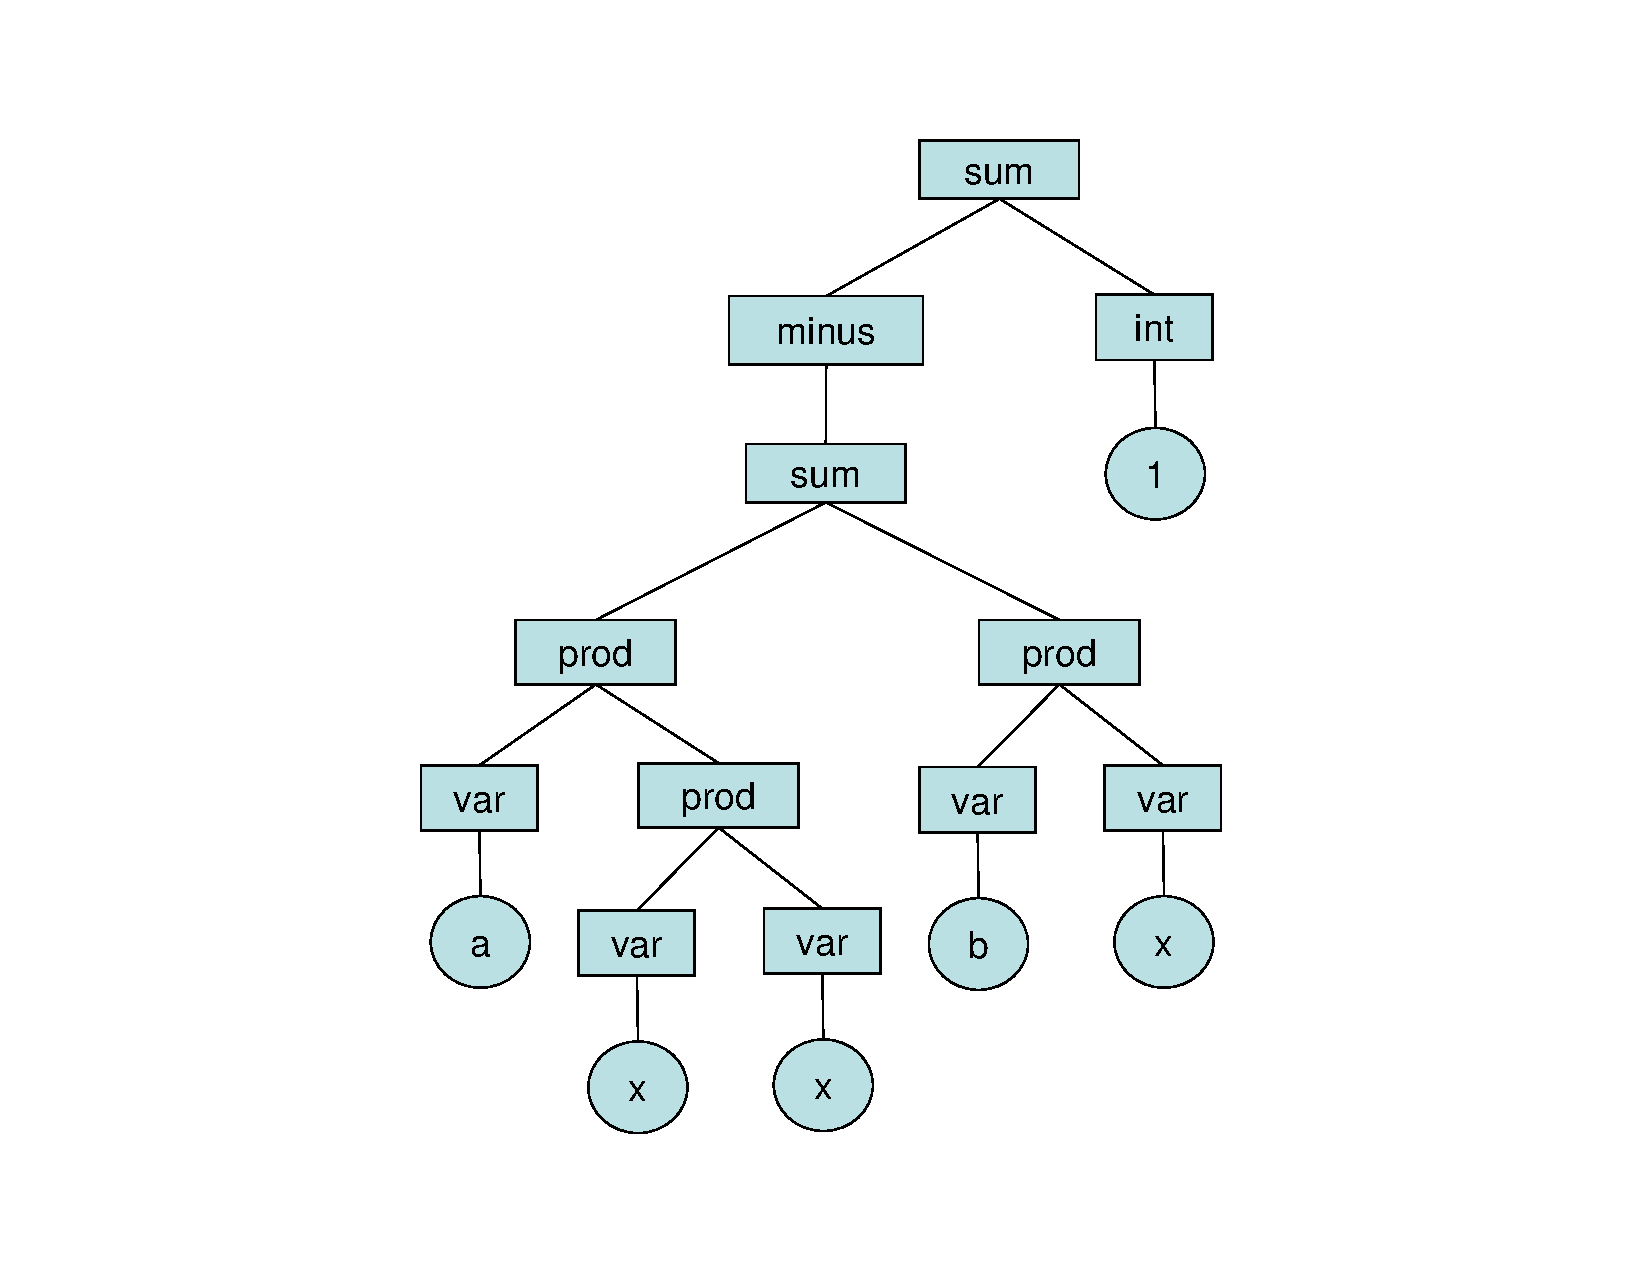
\includegraphics[width=5in]{parsetree}
\caption{Parse tree for $-(a(x\cdot x)+ bx) + 1$.}
\label{fig:parse}
\end{figure}

In a computer, such a tree would be represented by pairs or triples
that begin with a
\emph{tag} equal to the label of the top node of the parse tree.  
The general definition of parse trees for $\aexp$'s would be:

%\newcommand{\paexp}{\text{Aexp-parse-tree}}

\begin{definition}\label{arithparse}
The set $\paexp$ of \emph{parse trees for arithmetic expressions} 
over a set of
\emph{variables} $V$ is defined recursively as follows:
\begin{itemize}
\item \inductioncase{Base cases}:
\begin{enumerate}
\item If $n \in \integers$, then $\ang{\texttt{int}, n} \in \paexp$.
\item If $v \in V$, then $\ang{\texttt{var}, v} \in \paexp$.
\end{enumerate}
\item \inductioncase{Constructor cases}: if $e,e' \in \paexp$, then
\begin{enumerate}
\item $\ang{\texttt{sum}, e, e'} \in \paexp$,
\item $\ang{\texttt{prod}, e, e'} \in \paexp$, and
\item $\ang{\texttt{minus}, e} \in \paexp$.
\end{enumerate}
\end{itemize}
\end{definition}

So the $\paexp$ corresponding to formula~\ref{ax} would be:
\begin{equation}\label{axtag}
\begin{array}{rll}
\left< \right. \texttt{sum}, 
         & \left< \right. \texttt{minus},\ \ \left< \right. \texttt{sum},
               & \ang{\texttt{prod},\ \ \ang{\texttt{var},\ a},
                                     \ang{\texttt{prod},\ \
                                            \ang{\texttt{var},\ x},\
                                            \ang{\texttt{var},\ x}}},\\
                               && \left. \left. \ang{\texttt{prod},\ \
                                       \ang{\texttt{var},\ b},\
                                       \ang{\texttt{var},\ x}}
                                   \right> \right>,\\
         & \left. \left. \ang{\texttt{int},\ 1} \right> \right>
\end{array}
\end{equation}
Now the expression~\ref{ax} is certainly a lot more humanly
intelligible than~\ref{axtag}, but~\ref{axtag} is in the
representation best suited and commonly used in compiling and
processing computer programs.

\end{editingnotes}

\classproblems
\pinput{CP_recursive_prop_form_eval}

\bparts

\ppart State some reasonable generalization of the Fundamental Theorem
to games with an infinite set $V$ of possible payoffs.
\emph{Optional}: Prove your generalization.

\begin{solution}
The obvious generalization would redefine the max-value as the lub of
the ensured values, and the min-value as the glb of the limits to
payoffs.  The result is that some games may now have a value $v$ that
is positive or negative infinity, and that $v$ can't exactly be
ensured or limted to, but rather that for any $\epsilon >0$ there will
be a strategy that ensures a value of at least $v - \epsilon$ and a
strategy that limits payoff to at most $v + \epsilon$.
\end{solution}


\subsection{Game Trees}
More generally, we can describe the possible ways a game of Nim can be
played with a \term{game tree}.  A game tree for the Nim game that
starts with three piles of 3, 4 and 5 stones, respectively, is shown
in Figure~\ref{fig:endgame}.  The game tree has a \term{root} node
labelled with the starting position $\ang{3,4,5}$.\footnote{Game trees
  are usually pictured in this way, with the root at the top and lines
  connecting down to children.  The ``leaves'' at which the paths
  going down from the root appear at the bottom---in Computer as in
  geneaology, trees grow upside down.}  The root node is connected to
\emph{child nodes} corresponding to the possible piles after one move.
For example, the first player can remove between one and three stones
from the first pile leading to three possible piles of stones
\[
\ang{2,4,5},\ang{1,4,5},\ang{4,5}.
\]
Similarly, the first player has five possible ways to remove stones
from the last pile, leading to five possible piles of stones
\[
\ang{3,4,4}, \ang{3,4,3}, \ang{3,4,2}, \ang{3,4,1}, \ang{3,4} nodes.
\]
Altogether, the root of this particular game will be connected to $3
\times 4 \times 5 = 60$ child nodes.

Each child node will now have grandchild nodes showing the possible
piles of stones after the second player moves.  For example, the child
node $\ang{3,4,1}$ will be connected to $3 \times 4 \times 1 = 12$
grandchild nodes.  A path following connections down from the root to
a leaf describes a complete \term{play} of the game.

\begin{figure}[htbp]
%\graphic{endgame}
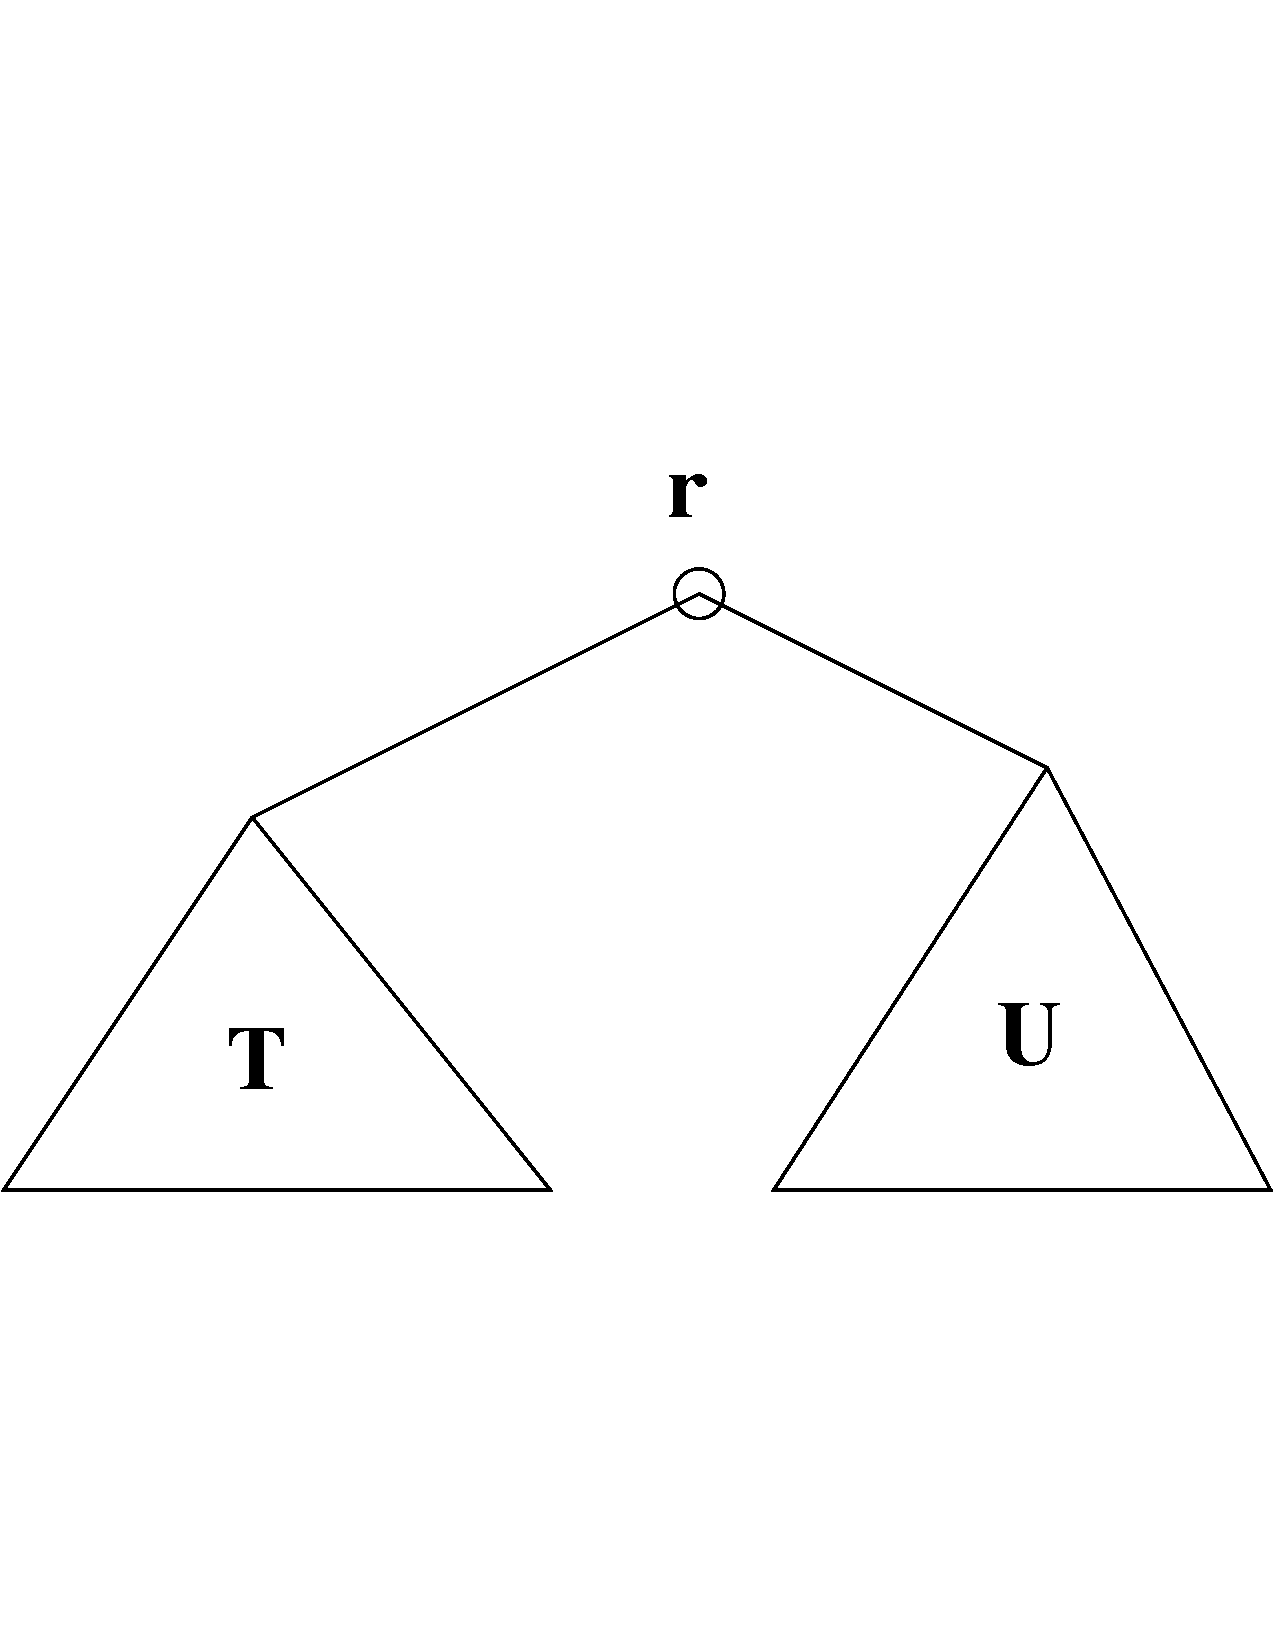
\includegraphics[width=6in]{recBST.pdf} %nimtree
\caption{\TBA{Game Tree for Nim starting with three piles of sizes $\ang{5,5,7}$}.}
\label{fig:endgame}
\end{figure}
\fi
